\lab{Algorithms}{Finite Volume Methods}{Finite Volume Methods}
\label{lab:finitevolume}

\section{Introduction to Conservation Laws}
We will focus on the conservation law
\begin{gather}\label{eq:1D_continuous}
u_t + f_x(u) = 0
\end{gather}
where for the purposes of this example, $u$ is a (spatially) one-dimensional conserved quantity, and $f(u)$ is the flux of $u$.  Before proceeding we note the following from the continuous version of the equation \eqref{eq:1D_continuous}
\begin{gather}
\frac{d}{dt}\int_a^b u(x,t) dx = 0
\end{gather}
when $u$ satisfies periodic boundary conditions on the interval $[a,b]$.  If the boundary conditions are not periodic, we note that the time evolution of the total `mass' or integral of $u$ across the domain, is dependent only on the flux through the boundaries, that is
\begin{gather}
\frac{d}{dt}\int u(x,t) dx = f(u(a))-f(u(b)).
\end{gather}

\begin{figure}[ht]
\centering
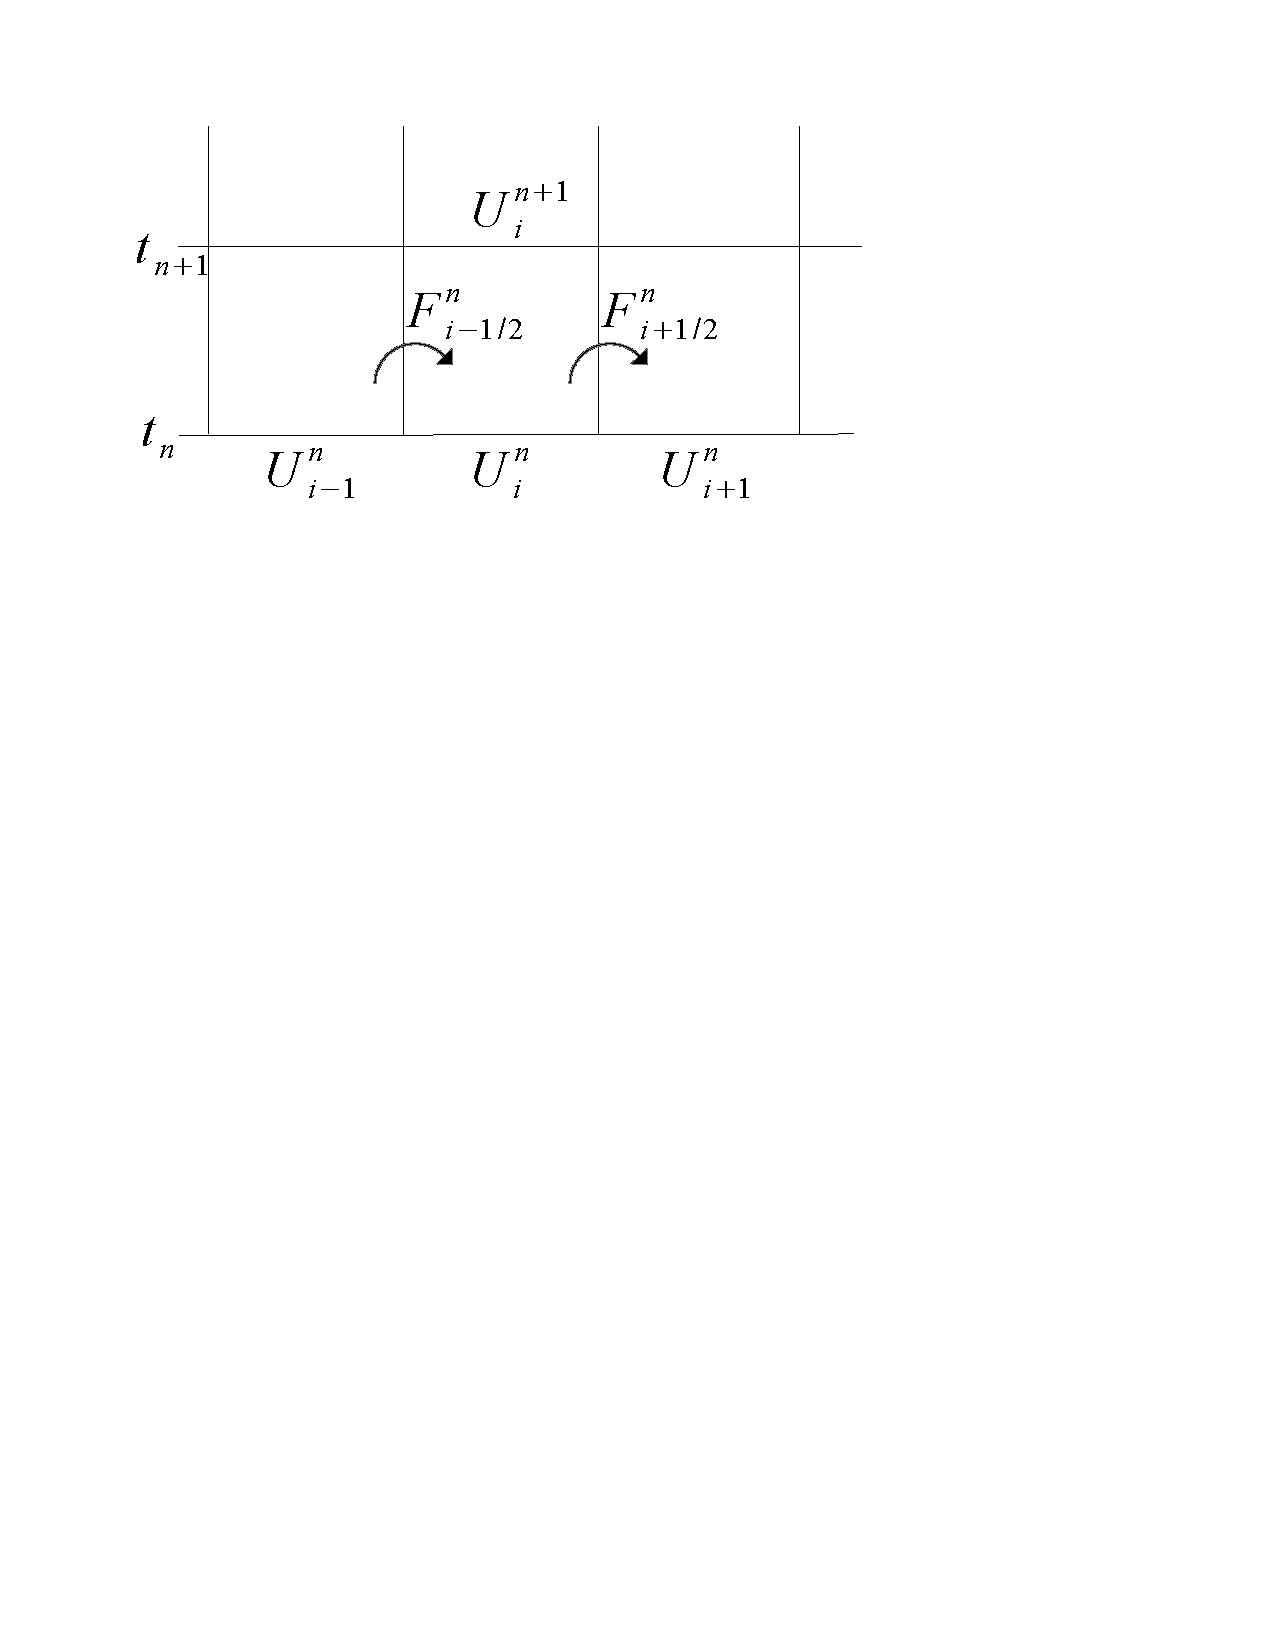
\includegraphics[trim= 20mm 195mm 0mm 30mm, clip]{flux_form.pdf}
\caption{A schematic of the fluxes for the finite volume method as indicated by \eqref{eq:flux_form}.}
\end{figure}

Finite volume methods are built around this premise, considering the evolution of $u$ not at a given point, but instead in volume averaged regions.  For example, given a typical finite difference discretization at points $x_i$ with standard spacing $\Delta x$ (generalizations to non-standard grid spacing are possible, just a bit more complicated), let $C_i$ be the i-th `volume' defined by $(x_{i-1/2},x_{i+1/2})$. then we are interested in the evolution of the volume average of $u$ over this interval,
\begin{gather}
U_i^n  = \frac{1}{\Delta x}\int_{C_i} u(x,t^n)dx
\end{gather}
where $t^n$ is the typical finite time discretization.  One of the motivations for doing this is that then the evolution of these volume averaged quantities will depend only on the flux through the cell edges, i.e. we can check easily enough that
\begin{gather}\label{eq:1D_semi_continuous}
\frac{d}{dt}\int_{C_i} u(x,t) dx = f(u(x_{i-1/2},t))-f(u(x_{i+1/2},t)).
\end{gather}
Thus, so long as the temporal discretization for the above is chosen wisely, we can ensure conservation of $\sum_i U_i^n\Delta x$ (the total `mass' of the system) from one time step $n$ to the next.  Thus, by integrating \eqref{eq:1D_semi_continuous} in time,we consider the evolution of the cell (`volume') averages as
\begin{gather}\label{eq:flux_form}
U_i^{n+1} = Q_i^n - \frac{\Delta t}{\Delta x} \left(F^n_{i+1/2}-F^n_{i-1/2}\right),
\end{gather}
where
\begin{gather}
F_{i-1/2}^n = \frac{1}{\Delta t} \int_{t_n}^{t_{n+1}}f(u(x_{i-1/2},t))dt. 
\end{gather}
This formulation guarantees the conservation properties that are so desirable for conservation laws, if the time-averaged fluxes $F_{i-1/2}^n$ can be discretized in a natural way.

\begin{problem}
Derive \eqref{eq:flux_form}.

\begin{align*}
\int_{t^n}^{t^{n+1}} \frac{d}{dt}\int{C_i} u(x,t)\, dx = \int_{t^n}^{t^{n+1}} \left[ f(u(x_{i-1/2},t)) - f(u(x_{i+1/2},t)) \right]
\end{align*}
\end{problem}

The key contribution of finite volume methods is the computation of $F_{i-1/2}^n$.  For a truly nonlinear $f(u)$ this can be rather complicated and messy, and typically will involve solving what is usually referred to as the Riemann problem for the conservation law.  We don't have the time to go there, but the interested student can look at \cite{Le2002} for a very thorough introduction and discussion on the subject.  Instead we will do what is always done in applied mathematics (which means everywhere) and consider the linear problem first in one-dimension.  The analog to higher dimensions can easily be seen by considering the eigenvector decomposition of any linear system.  The connection to the full nonlinear equation is a bit more complicated, but is reserved for another course.

\section{The linear advection equation and upwinding}
The simplest conservation law is simply advection of a quantity
\begin{gather}
u_t + au_x = 0,
\end{gather}
which describes the advection or movement of a concentration of some constituent by a constant velocity one-dimensional `wind' $a$ (a slight generalization of this would be to consider $a=a(x)$, but the general concepts are exactly the same as those viewed here, just a more local consideration is necessary).  In higher dimensions this is an important problem in many fields, for example the transport of chemicals in the atmosphere and oceans, proper mixing of various properties in metallurgy, and the passing of information along a network.

One of the most useful properties of the advection equation is that if $u(t,x)$ is a solution of this equation, then so is $u(x-at,t)$, that is if $u(x,0) = u_0(x)$ then the solution for all time can be represented by $u(x,t) = u_0(x-at)$.  This also gives a new meaning to the term advection, i.e. all that this equation does is takes the initial conditions and passively transports them with velocity $a$.

In this case, the computation of the flux appears straightforward, $F_{i-1/2}^n = a\overline{U}^n_{i-1/2}$ where the $\overline{\cdot}$ refers to the time average over the interval $t_n$ to $t_{n+1}$.  We still need to determine how to approximate this time average however.  To understand how this might be done, note from Fig. \ref{something} that for the advection equation with $a>0$ the flux that determines $U_i^{n+1}$ will be dependent on the value of $U_{i-1}^n$ so that it makes sense that we approximate the flux here as $F_{i-1/2}^n = aU_{i-1}^n$ (recall that the $U_i^n$ are cell averages of the continuous quantity $u(x)$).  Similarly if $a<0$ then $F_{i-1/2}^n = aU_{i}^n$.  This is called the first order upwind method and gives a completely discretized version of the problem as \eqref{eq:flux_form} with
\begin{gather}
F_{i-1/2}^n = a^- U_i^n + a^+U_{i-1}^n,
\end{gather}
where $a^- = \min (a,0)$ and $a^+ = \max (a,0)$.  Note that this formulation allows for an easy extension to the case of $a=a(x)$.  From now on we will consider $a>0$ only, the generalization to other cases is relatively straightforward.

\begin{figure}[ht]
\centering
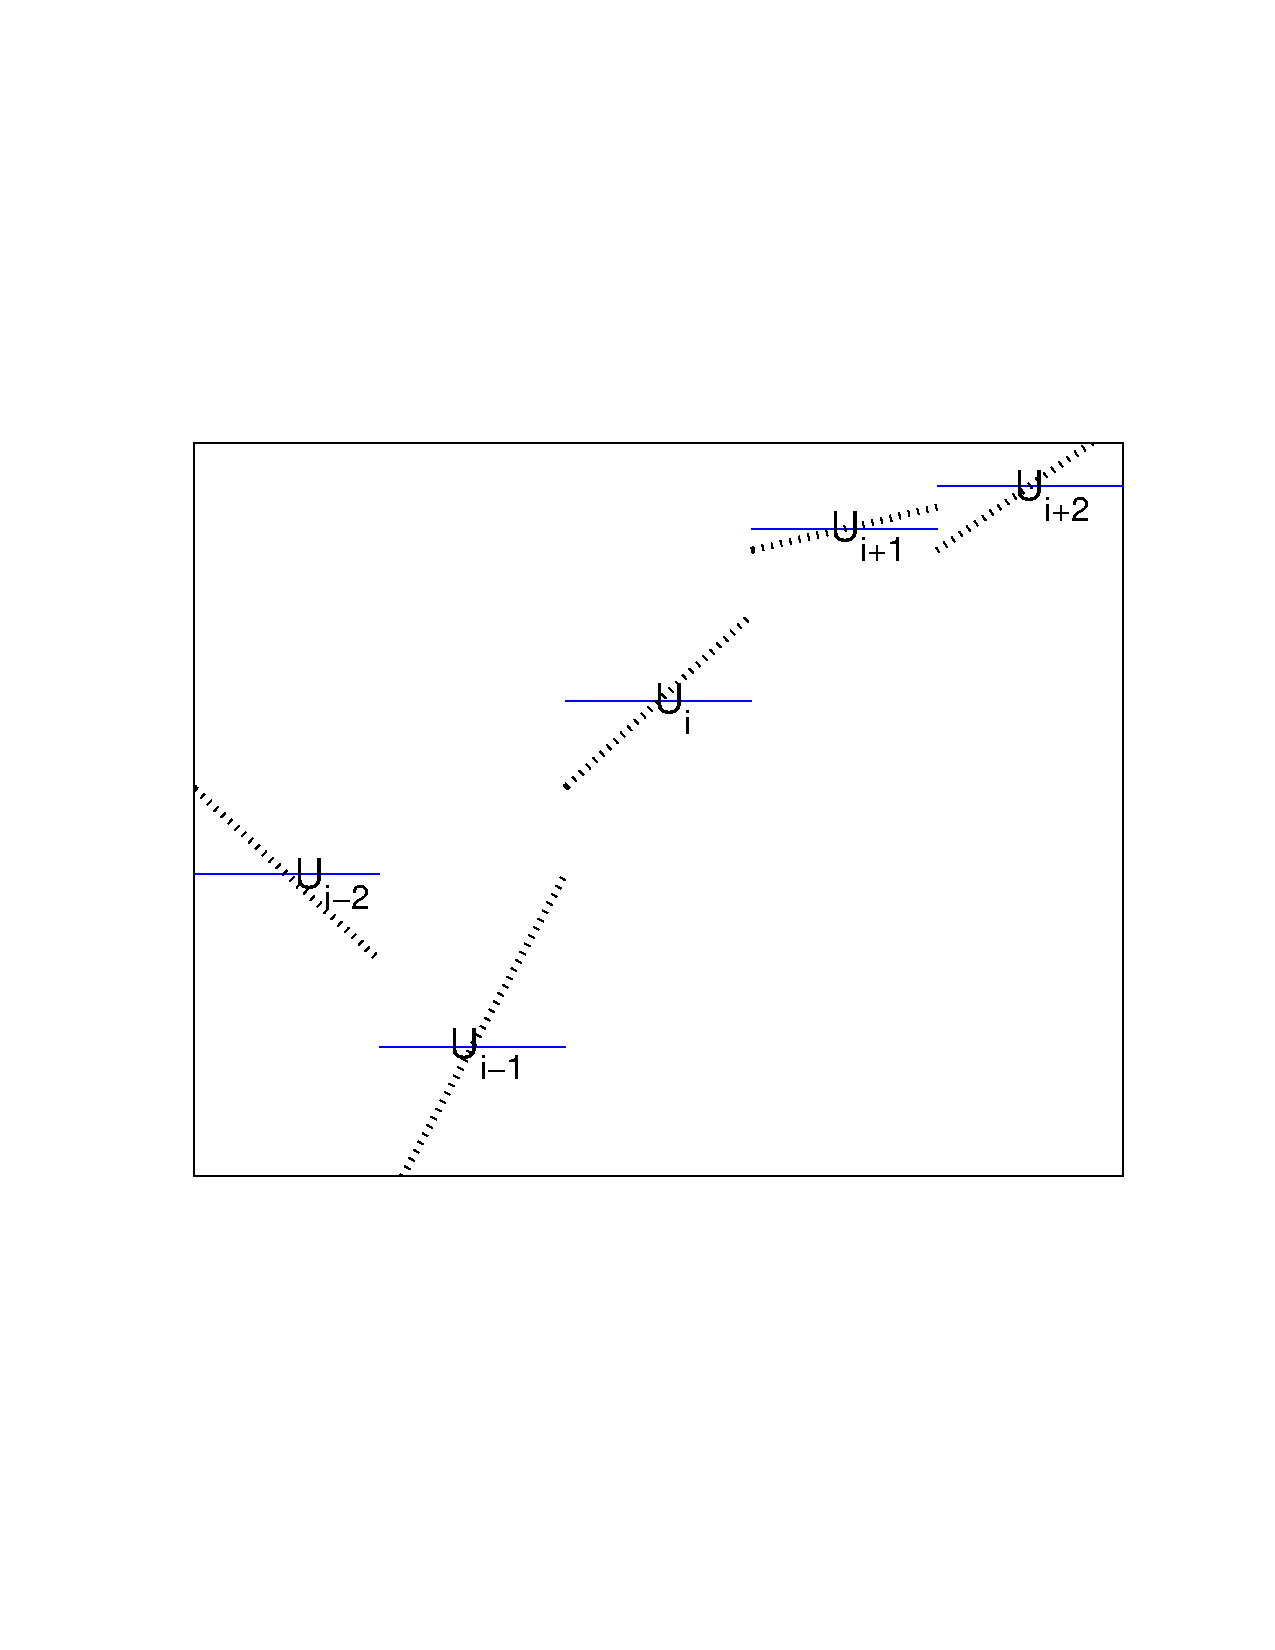
\includegraphics[width=\textwidth, trim = 20mm 65mm 20mm 65mm, clip]{LW_reconstruction.pdf}
\caption{The piecewise linear reconstruction for the upwind and Lax-Wendroff methods.  The solid lines represent the simplest reconstruction of the cell averages leading to the upwind method, and the dashed lines are those whose slope is obtained via the Lax-Wendroff method.  Note that the LW method introduces a spurious maximum at $i+3/2$ (the cell edge between $U_{i+1}$ and $U_{i+2}$) and the minimum at $i-3/2$ will be unphysical exaggerated.  The upwind method avoids this difficulties, but clearly loses a significant amount of the available information.  This provides the motivation for the slope limiters.}
\end{figure}

Another way to derive the upwind method is to instead suppose that what we want to do is reconstruct $u(x)$ at each time step $n$ inside each cell $(x_{i-1/2},x_{i+1/2})$ from the mean values in that cell and its surrounding neighbors.  This reconstructed $\tilde{u}(x)^n$ is then defined piecewise for each cell $i$.  The solution at the next time step can be found as $\tilde{u}^{n+1}(x) = \tilde{u}^n(x-a\Delta t)$ which allows us to determine the fluxes $F_{i-1/2}^n$ once we have settled on a method for determining $\tilde{u}^n(x)$ in each cell.  The simplest approach is
\begin{gather}
\tilde{u}^n(x) = U^n_i \mbox{ for } x \in (x_{i-1/2},x_{i+1/2}).
\end{gather}
This leads to fluxes given by
\begin{gather}
F_{i-1/2}^n = \frac{a}{\Delta t} \int_{t_n}^{t_{n+1}}\tilde{u}(x_{i-1/2}-a(t-t_n),t)dt = \frac{a}{\Delta t} \int_{t_n}^{t_{n+1}}U_i^n dt = aU_i^n.
\end{gather}
In either case, we can see that using the flux differencing formula \eqref{eq:flux_form} that
\begin{gather}
U_i^{n+1} = U_i^n - \frac{a\Delta t}{\Delta x}\left(U_i^n-U_{i-1}^n\right)
\end{gather}
for the upwind method.

\section{Piecewise linear reconstruction and slope limiters}
The upwind method is formally only first order, and actually does relatively poorly in terms of actually transporting the initial data with velocity $a$.  You can notice from the example code that the upwind method has errors that are `diffusive' meaning that the initial data is diffused as time evolves, losing the peaks and fine details.  This is because the error for the upwind method is on the order of the second derivative of $u$ which is of a diffusive nature.  To get an improved method, consider a better reconstruction inside each cell, i.e.
\begin{gather}
\tilde{u}^n(x) = U_i^n + m_i^n(x-x_i) \mbox{ for } x \in (x_{i-1/2},x_{i+1/2})
\end{gather}
where the slope of this linear reconstruction $m_i^n$ is determined as a function of the neighboring cell averages at time $n$ and $U_i^n$ itself.  One of the most natural approaches is to just estimate the slope depending on the cell $i$ and a neighboring cell $i+1$ or $i-1$.  This leads to two popular methods, respectively the Lax-Wendroff method (which we consider explicitly here) and the Beam-Warming method (that really is the name I promise).  The Lax-Wendroff method has a slope chosen as
\begin{gather}
m_i^n = \frac{U^n_{i+1}-U_{i-1}^n}{\Delta x}.
\end{gather}
This leads to
\begin{gather}
U_i^{n+1} = U_i^n - \frac{\Delta t}{2\Delta x} a \left(U_{i+1}^n-U_{i-1}^n\right) + \frac{1}{2}\left(\frac{\Delta t}{\Delta x}\right)^2 a^2 \left(U_{i-1}^n - 2U_i^n+U_{i+1}^n\right)
\end{gather}
which it turns out is formally second-order accurate.  It turns out though that the errors for this method are dispersive, meaning that near very steep gradients, the method will generate very rapid oscillations (due to the third derivative of $u$ not being approximated accurately).  Another way to consider how these errors arise is to notice from Fig. \ref{something here} that if the piecewise linear reconstruction is advocated by some positive wind $a$ then there will be places where the discontinuous nature of the reconstruction will introduce spurious maxima or minima into the solution.  These become the spurious waves seen simulations via the Lax-Wendroff method.

A solution to this dilemma between balancing the diffusive and dispersive errors comes from constructing slopes $m_i^n$ that ensure no such non-monotonic transport takes place.  Several examples are given below, but the basic idea is to constrain the slope so that the reconstructed piecewise linear function $\tilde{u}^n(x)$ will not generate unphysical extremal values when it is advocated by some finite wind $a$.

\begin{itemize}
\item Minmod limiter
\begin{gather}
m_i^n = minmod\left(\frac{U_i^n-U_{i-1}^n}{\Delta x},\frac{U_{i+1}^n-U_{i^n}}{\Delta x}\right)
\end{gather}
where
\begin{gather}
minmod(a,b) = \left\{\begin{array}{ccc}a  \mbox{ if } |a| < |b|  \mbox{ and } ab>0\\
b  \mbox{ if } |b|<|a|  \mbox{ and } ab>0\\ 0  \mbox{ if } ab < 0 .\end{array}\right.
\end{gather}
\item Superbee limiter
\begin{gather}
m_i^n = maxmod(m^{(1)}_i,m^{(2)}_i)
\end{gather}
where the maxmod function selects $m^{(k)}_i$ with the larger modulus, and
\begin{gather}
m^{(1)}_i = minmod \left(\frac{U_{i+1}^n-U_i^n}{\Delta x},2\frac{U_i^n-U_{i-1}^n}{\Delta x}\right)\\
m^{(2)}_i = minmod \left( 2\frac{U_{i+1}^n-U_i^n}{\Delta x},\frac{U_i^n-U_{i-1}^n}{\Delta x}\right).
\end{gather}
\item Monotonized central-difference limiter
\begin{gather}
m_i^n = minmod\left(\frac{U_{i+1}^n-U_{i-1}^n}{2\Delta x},2\frac{U_i^n-U_{i-1}^n}{\Delta x},2\frac{U_{i+1}^n-U_i^n}{\Delta x}\right)
\end{gather}
\end{itemize}

\begin{problem}
Code up the Superbee and MC limiters for an advection problem with constant wind.  Use different initial data that is smooth or has steep gradients (such as the square wave in the example code) to see which of the three limiters may be more optimal.
\end{problem}

\section{Beyond piecewise linear reconstructions}
As you can imagine, using a linear approximation is not the only option.  There are a host of high order finite volume methods that consider polynomial reconstructions of $\tilde{u}^n$ inside each cell.  The key is then to use some nonlinear limiting technique that will ensure that when $\tilde{u}^n(x)$ is advocated that no new extrema are introduced.  Choosing the correct limiter for the given application then becomes an art unto itself.